\documentclass{beamer}

% There are many different themes available for Beamer. A comprehensive
% list with examples is given here:
% http://deic.uab.es/~iblanes/beamer_gallery/index_by_theme.html
% You can uncomment the themes below if you would like to use a different
% one:
%\usetheme{AnnArbor}
%\usetheme{Antibes}
%\usetheme{Bergen}
%\usetheme{Berkeley}
%\usetheme{Berlin}
%\usetheme{Boadilla}
%\usetheme{boxes}
%\usetheme{CambridgeUS}
%\usetheme{Copenhagen}
%\usetheme{Darmstadt}
%\usetheme{default}
%\usetheme{Frankfurt}
%\usetheme{Goettingen}
%\usetheme{Hannover}
%\usetheme{Ilmenau}
%\usetheme{JuanLesPins}
%\usetheme{Luebeck}
\usetheme{Madrid}
%\usetheme{Malmoe}
%\usetheme{Marburg}
%\usetheme{Montpellier}
%\usetheme{PaloAlto}
%\usetheme{Pittsburgh}
%\usetheme{Rochester}
%\usetheme{Singapore}
%\usetheme{Szeged}
%\usetheme{Warsaw}
\setbeamertemplate{caption}[numbered]
\usepackage{array}
\usepackage[utf8]{inputenc}
\usepackage[russian]{babel}
\usepackage{amsmath}
%\title{Расчет спектра электрона в сферически симметричных потенциалах}
\newcommand{\mi}{\mathrm{i}}
\DeclareMathOperator\supp{supp}
\DeclareMathOperator\rect{rect}
\usepackage{algorithm}
\usepackage{algpseudocode}
%\author{Е.Г. Орлова, 3 курс\\
%департамент Прикладной математики НИУ ВШЭ\\
%Научный руководитель: Р.Ш. Ихсанов, доцент\\
%департамент Электронной инженерии НИУ ВШЭ
%}
% - Give the names in the same order as the appear in the paper.
% - Use the \inst{?} command only if the authors have different
%   affiliation.

\usepackage{float}
\usepackage{caption}
\usepackage{subcaption}
\usepackage{graphicx}

\author[E. Orlova]{Е.Г. Орлова, 3 курс\\
департамент Прикладной математики НИУ ВШЭ \vskip 2 mm
Научный руководитель: Р.Ш. Ихсанов, доцент\\
департамент Электронной инженерии НИУ ВШЭ}
\title[Расчет спектра электрона]{Расчет спектра электрона в сферически симметричных потенциалах}
% Let's get started
\begin{document}

\begin{frame}
  \titlepage
\end{frame}

\begin{frame}{Постановка задачи}

	\begin{itemize}
        \item Найти решение стационарного уравнения Шредингера для сферически симметричных потенциалов (потенциальная энергия частицы зависит только от расстояния между частицей и центром).
        \item Найти спектр – решить задачу на собственные значения вида:
       
         $$(-\frac{\hbar^2}{2m}\frac{d^2 }{d r^2}+[V+\frac{\hbar^2}{2m}\frac{l(l+1)}{r^2}])u = Eu.$$
         Задача редко имеет аналитическое решение.
       
	 \end{itemize}

\end{frame}


\begin{frame}{Численные методы}
Для решения задачи на собственные значения применен метод конечных разностей.
   \vskip 2mm
    \begin{itemize}
    		\item Использовалась разностная аппроксимация второго порядка:
    		$$\displaystyle{{u_n''} = \frac{u_{n+1}-2u_n +u_{n-1}}{h^2}};$$  
    		$$\begin{bmatrix}
u_1'' \\
u_2'' \\
u_3'' \\
\vdots \\
u_n''
\end{bmatrix} = \frac{1}{h^2} \begin{bmatrix}
-2 & 1 &0&0&0& \cdots & 0 \\
1 & -2 & 1& 0&0&\cdots & 0 \\  
0&1 & -2 & 1& 0&\cdots & 0 \\  
\vdots & \vdots &\vdots & \vdots & \ddots & -2& 1  \\
0 & 0&0 &0& \cdots &1 & -2
\end{bmatrix}
\begin{bmatrix}
u_1
\\
u_2
\\
u_3
\\
\vdots
\\
u_n
\end{bmatrix}. $$
  
   \end{itemize}
    
\end{frame}


\begin{frame}{Граничные условия}
	 Волновая функция обычно экспоненциально затухает, поэтому с вычислительной точки зрения можно считать, что $u (r) = 0$ при $ r \geq L$ для некоторого большого $L$.\\
	Мы получаем задачу на собственные значения с граничными условиями $u (0) = 0$ (так как$ u (r) = r R (r)$) и $u (L) = 0$.
\end{frame}


\begin{frame}{Численные методы}
Экстраполяция Ричардсона: \vskip 2mm
$$E_{N} - E = C (2h)^2,$$
$$E_{2N} - E = C h^2,$$
\vskip 2mm
 $$E = \frac{4 E_N - E_{2N}}{3}.$$
 \vskip 2mm
 Также использовался метод Ньютона.
  
\end{frame}

\begin{frame}{Тестирование численного решения на известные аналитические результаты}
  Для потенциальной ямы конечной глубины $$V(r)=\begin{cases}
-V_0, ~\text{if } r< R\\
~~~~0, ~\text{if } r>R
\end{cases}$$
решение при $l = 0$ задается следующей формулой: 
$$\tan(\sqrt{2} a \sqrt{V_0-E})=-\sqrt{\frac{V_0}{E}-1}.$$ 
\end{frame}


\begin{frame}{Результаты для потенциальной ямы конечной глубины}

\begin{figure}[h!]
\centering
\begin{subfigure}{.5\textwidth}
  \centering
  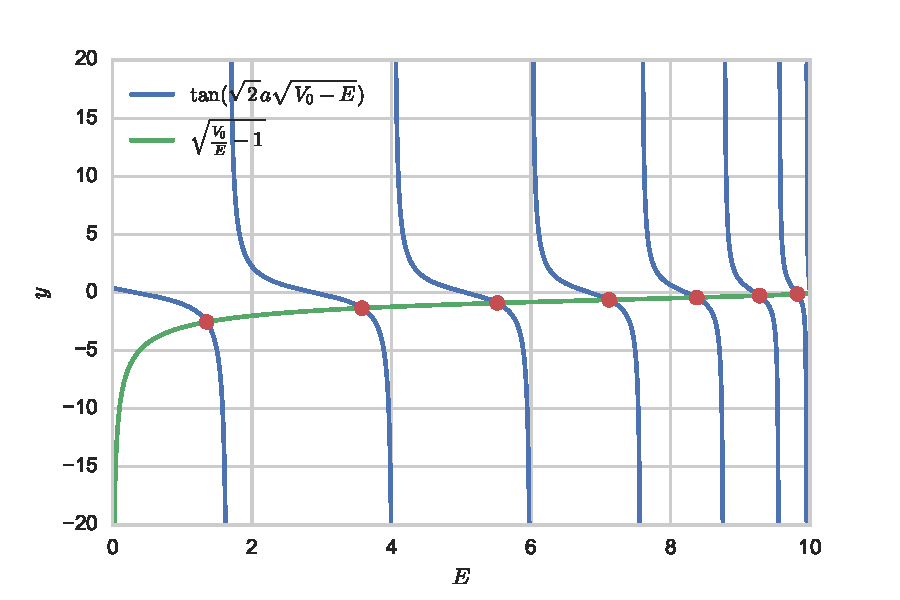
\includegraphics[width=1.0\linewidth]{tan-sqrt.pdf}
  \caption{$\tan(\sqrt{2} a \sqrt{V_0-E})=-\sqrt{\frac{V_0}{E}-1}$}
  \label{fig1:tan-sqrt}
\end{subfigure}%
\begin{subfigure}{.5\textwidth}
  \centering
  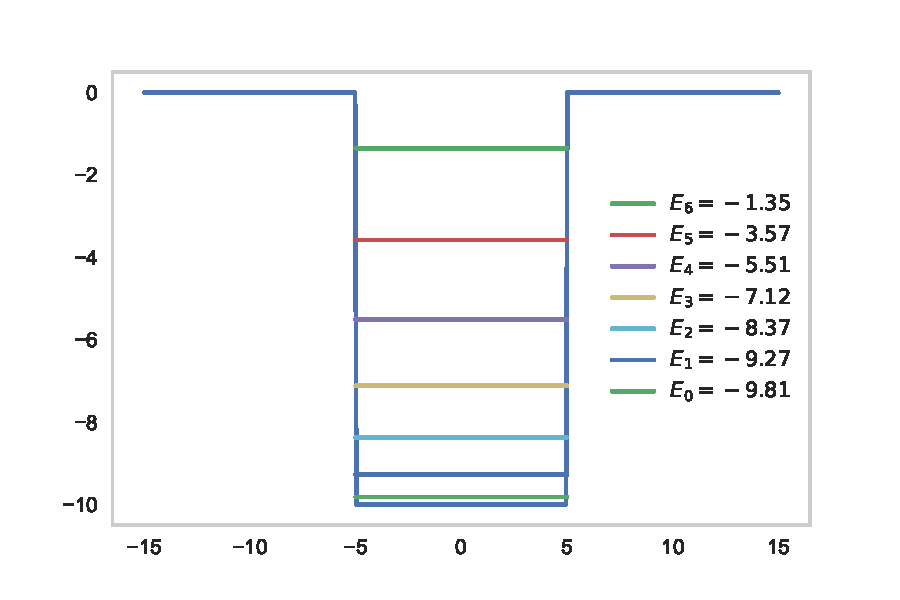
\includegraphics[width=1.0\linewidth]{ens_finite.pdf}
  \caption{Значения спектра (а. е.)}
  \label{fig:finite_well_sol}
\end{subfigure}
\caption{Потенциальная яма конечной глубины}
\label{fig:fin_well}
\end{figure}
  
\end{frame}

\begin{frame}{Гармонический осциллятор}
 Потенциал для гармонического осциллятора задается
$$V(r) = \frac{1}{2} m \omega^2 r^2.$$
Аналитическое решение для спектра известно:
$$E_{nl} = \hbar \omega (2 n+l+\frac{3}{2}),~~ n = 0,~1,~2,...$$
\end{frame}

\begin{frame}{Результаты для гармонического осциллятора}
\begin{table}
\parbox{.45\linewidth}{
\centering
\begin{tabular}{l | c | c   }
n & Численное & Аналитическое \\
\hline \hline
$ 0 $&   0.5196\textcolor{red}{08} &    0.519615 \\
$ 1 $ &   1.21239\textcolor{red}{8} &    1.212436 \\
$ 2$ &   1.905\textcolor{red}{165} &    1.905256 \\
$ 3 $ &   2.5979\textcolor{red}{07} &    2.598076 \\
$ 4$ &   3.290\textcolor{red}{626} &    3.290897 \\
$ 5 $ &   3.983\textcolor{red}{320} &    3.983717 \\
\end{tabular}
\caption{$l=0$}
}
\hfill
\parbox{.45\linewidth}{
\centering
\begin{tabular}{l | c | c   }
n & Численное & Аналитическое \\
\hline \hline
0 &   0.8660\textcolor{red}{16} &    0.866025 \\
1 &   1.5588\textcolor{red}{07} &    1.558846 \\
2 &   2.25157\textcolor{red}{4} &    2.251666 \\
3 &   2.944\textcolor{red}{318} &    2.944486 \\
4 &   3.637037 &    3.637307 \\
5 &   4.3297\textcolor{red}{32} &    4.330127 \\
\end{tabular}
\caption{$l = 1$}
}
\caption{Возможные значения энергии для гармонического осциллятора}
\end{table}
\end{frame}


\begin{frame}{Иллюстрация для осциллятора}
\begin{figure}[h!]
\centering
\begin{subfigure}{.5\textwidth}
  \centering
  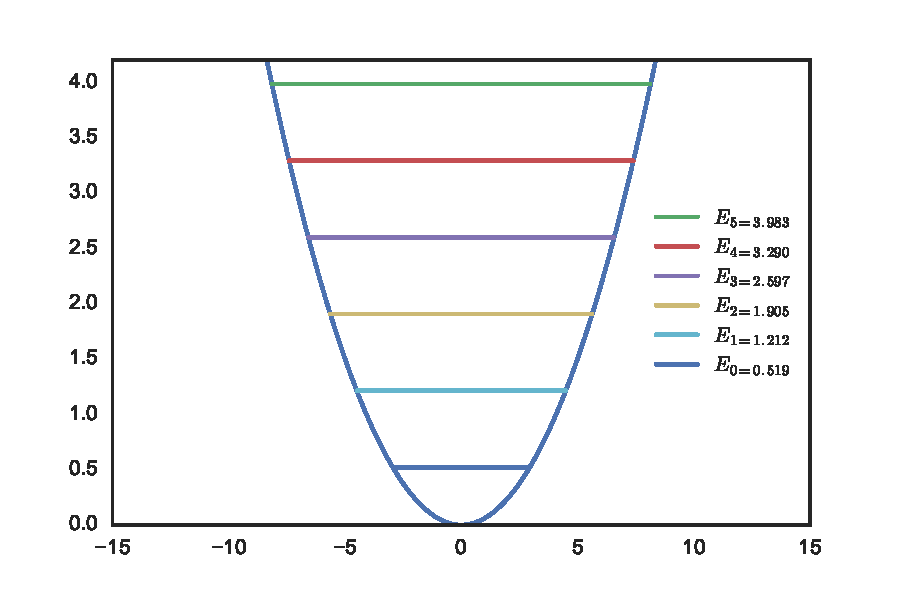
\includegraphics[width=1.0\linewidth]{harm_osc.pdf}
  \caption{$l = 0$}
  \label{fig1:tan-sqrt}
\end{subfigure}%
\begin{subfigure}{.5\textwidth}
  \centering
  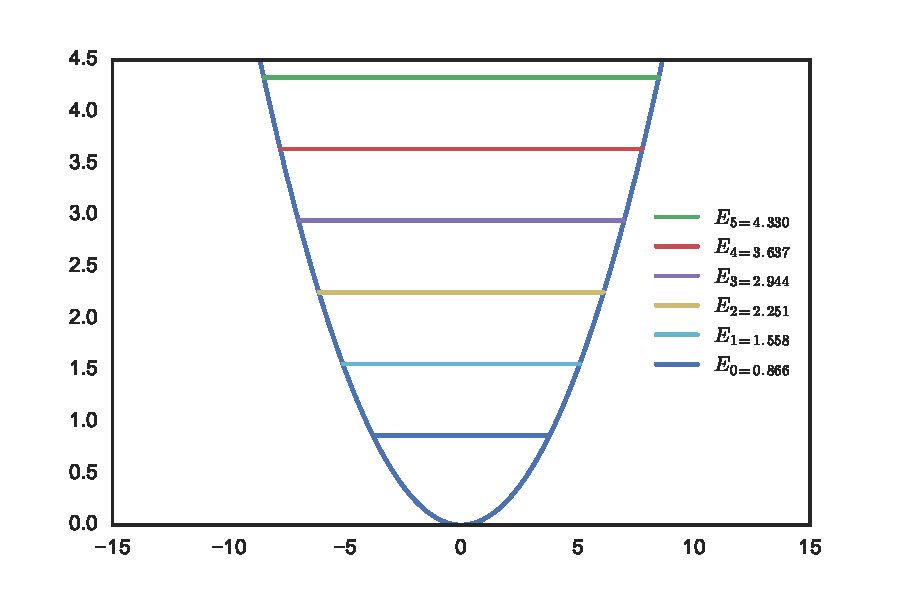
\includegraphics[width=1.0\linewidth]{harm_osc1.pdf}
  \caption{$l=1$}
  \label{fig:finite_well_sol}
\end{subfigure}
\caption{Гармонический осциллятор}
\label{fig:fin_well}
\end{figure}

\end{frame}

\begin{frame}{Атом водорода}
Потенциал в атомных единицах задается
$$V(r) = -\frac{1}{r}.$$
Аналитическое решение для спектра известно:
$$E_n = -\frac{1}{2 n^2},~~ n = 0,~1,~2,...$$

\end{frame}



\begin{frame}{Результаты для атома водорода}

\begin{figure}[h!]
\centering
\begin{subfigure}{.2\textwidth}
  \centering
  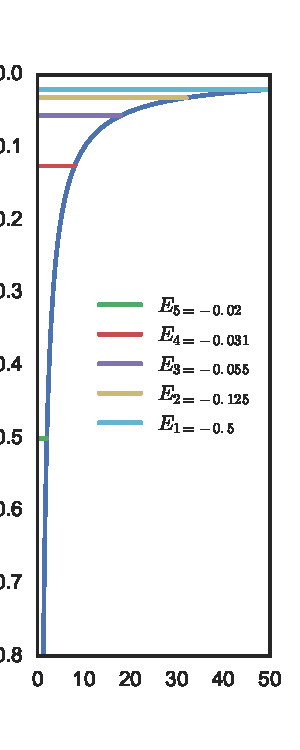
\includegraphics[width=1.0\linewidth]{h2_atom.pdf}
\end{subfigure}
\caption{Спектр атома водорода в а. е.}
\label{fig:h2_spectrum}

\end{figure}
\end{frame}

\begin{frame}{Результаты для атома водорода}
\begin{table}
\begin{tabular}{l | c | c   }
n & Численное & Аналитическое \\
\hline \hline
1 & -0.4999\textcolor{red}{11}& -0.500000 \\
2 & -0.12499\textcolor{red}{4} & -0.125000 \\
3 & -0.05555\textcolor{red}{4} & -0.055556 \\
4 & -0.031250 & -0.031250 \\
5 & -0.020000 & -0.020000 \\
\end{tabular}
\caption{Результаты для кулоновского потенциала в а. е.}
\end{table}
\end{frame}


\begin{frame}{Анализ сходимости метода}
 \begin{figure}[h!]
\centering
\begin{subfigure}{.8\textwidth}
  \centering
  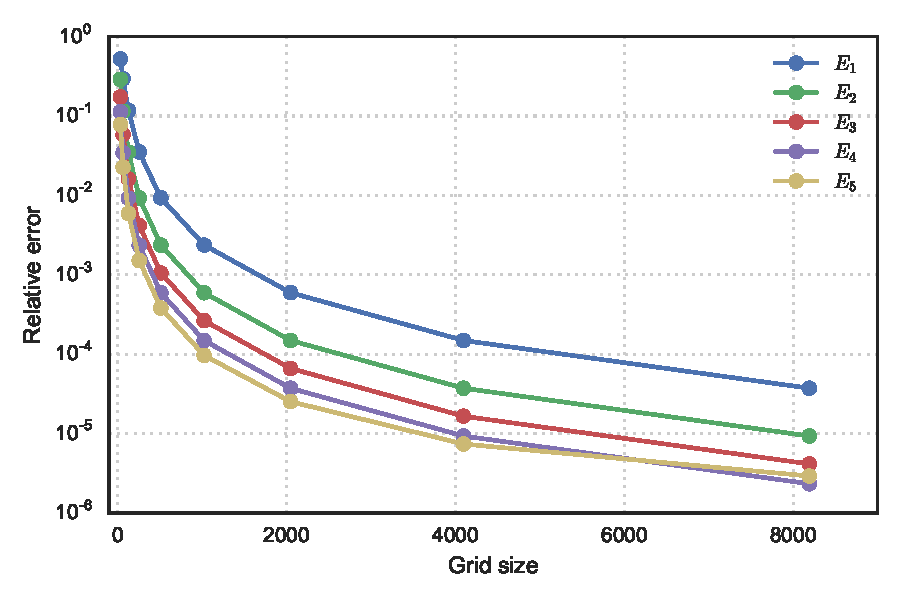
\includegraphics[width=1.0\linewidth]{h2_grid.pdf}
\end{subfigure}
\caption{Сходимость метода для кулоновского потенциала}
\end{figure}
\end{frame}




\begin{frame}{Результаты}
 \begin{itemize}
    		\item Разработаны и реализованы численные методы для расчета спектра электрона в сферически симметричных потенциалах.
    		\item Численные методы протестированы на известные аналитические решения или результаты других численных методов.
    		
   \end{itemize}
\end{frame}

\begin{frame}{Перспективы}
 \begin{itemize}
    		\item Реализованные программы будут использованы в образовательном процессе магистерской программы " Материалы. Приборы. Нанотехнологии."
    		\item Планируется публикация в журнал “Journal of chemical education”.
    		\item Планируется продолжение темы в рамках НУГ “Математическое моделирование квантовых приборов и материалов” (Л.Н. Щур, М.Ю. Каган, Е.А. Буровский, Р.Ш. Ихсанов) в случае поддержки проекта.
    		\vskip 4 mm
    		\centering{
    		\textbf{Спасибо за внимание!}}
   \end{itemize}
\end{frame}

%\begin{frame}{Конец}
%Спасибо за внимание!
%\end{frame}


% Emacs 24.3.50.2 (Org mode 8.2.3c)
\end{document}
